% !TeX spellcheck = da_DK
\section{Sensorer}
Følgende afsnit vil undersøge de sensorer der er til rådighed og som er interessanten for projektet.
Da der er stor forskel på sensorerne der er tilrådighed er der foretaget forskellige forsøg, hvis formål er at klarlægge præcisionen af de forskellige sensorer.

\begin{figure}[h]
\centering
\begin{subfigure}[b]{.4\textwidth}
\centering
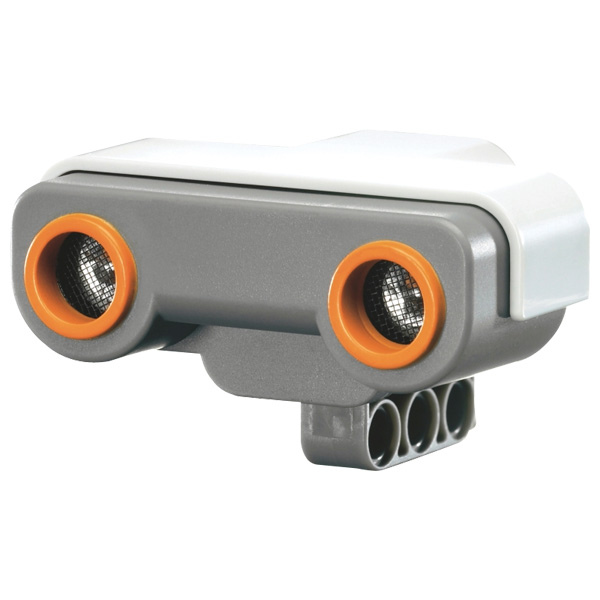
\includegraphics[width=.5\textwidth]{us}
\caption{Ultrasonisk sensor}
\label{sensor:ultrasonic_sensor}
\end{subfigure}
\begin{subfigure}[b]{.4\textwidth}
\centering
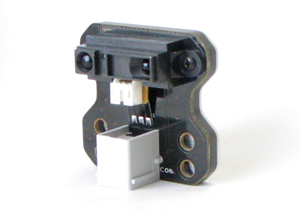
\includegraphics[width=.5\textwidth]{infrared_sensor}
\caption{Infrarød sensor}
\label{sensor:infraroed_sensor}
\end{subfigure}
\begin{subfigure}[b]{.4\textwidth}
\centering
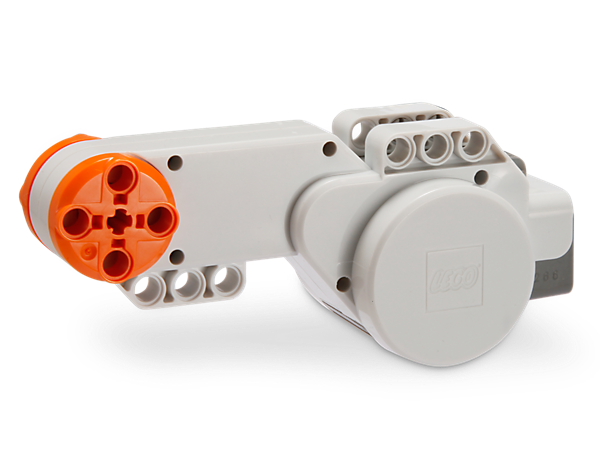
\includegraphics[width=.5\textwidth]{lego_motor}
\caption{Servomotor}
\label{sensor:servo_motor}
\end{subfigure}
\begin{subfigure}[b]{.4\textwidth}
\centering
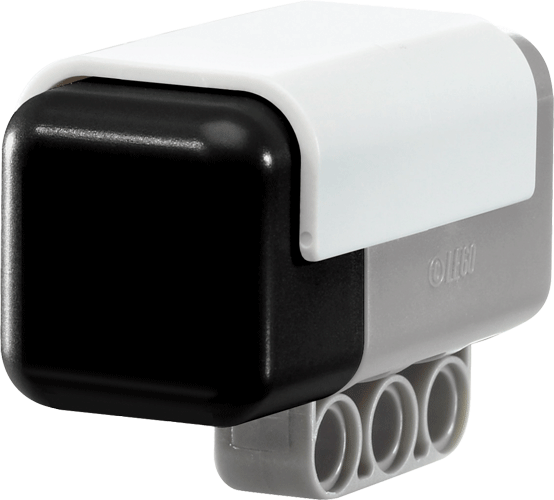
\includegraphics[width=.5\textwidth]{hitechnic_compass}
\caption{Kompas}
\label{sensor:compass}
\end{subfigure}
\end{figure}


\subsection{Ultrasonic Sensor}
Ultrasonic sensoren, som kan ses på \cref{sensor:ultrasonic_sensor}, er en sensor der kan måle afstand til objekter.

Det gøres ved at sende en lydbølge, hvorefter der beregnes hvor lang tid det tager for denne at ramme objektet, for derefter at blive reflekteret tilbage igen.
Sensoren måler afstanden i cm eller tommer.
Den maksimale afstand der kan måles er 255 cm med en præcision på $\pm$3 centimeter.
De bedste aflæsninger fås ved måling af store flade objekter med hård overflade, i modsætning til mindre objekter med rund og/eller blød overflade.\cite{nxt}

\subsubsection{Formål}
Formålet med at teste denne sensor er, at robotten skal have en måde at afgøre på, hvor langt der er til objekter omkring den.
Derfor vil denne test undersøge følgende:
\begin{itemize}
\item Hvor nøjagtigt kan denne sensor bestemme afstanden til et objekt?
\item Hvilket interval kan der måles i, hvad er den minimale og maksiamle måleafstand?
\end{itemize}

\subsubsection{Test}
Der er gennemført en mindre test af sensoren, for at finde ud af hvor nøjagtig den er.

Testen blev udført ved at lave en simpel konstruktion kun bestående af NXT og den ultrasoniske sensor.
Konstruktionen blev placeret i en række afstande fra en væg, hvor sensoreren var placeret vandret, pegende direkte på væggen.
Herefter blev sensoren aflæst, samtidig med at afstanden mellem væg og sensor blev målt med lineal.

\subsubsection{Resultater} Tabel med resultater fra forsøget kan ses i \cref{appendix:ultrasonisk}.

En graf-repræsentation af resultaterne kan ses i \cref{sensor:ultrasonic_resultat_diagram}.
Den røde linje indikerer det ideele resultat mens den blå, brune og grønne linje viser de resultaterne fra de tre test.
Det ses på grafen at de tre tests alle giver forkerte resultater når sensoren er mindre en 20 cm fra objektet.
Desuden kan det ses at der i test1 kun kunne måles op til 170 cm før der opstod usikkerhed, hvor de andre tests nåede 200 (test2) og 230 (test3) cm før der opstod større usikkerhed.
Generelt holder det som der bliver lovet, nemlig at der er en afvigelse på 3 cm på målingerne, men forsøget viser at der kun med sikkerhed kan måles mellem 20 og 170 cm.

\begin{figure}[h]
\centering
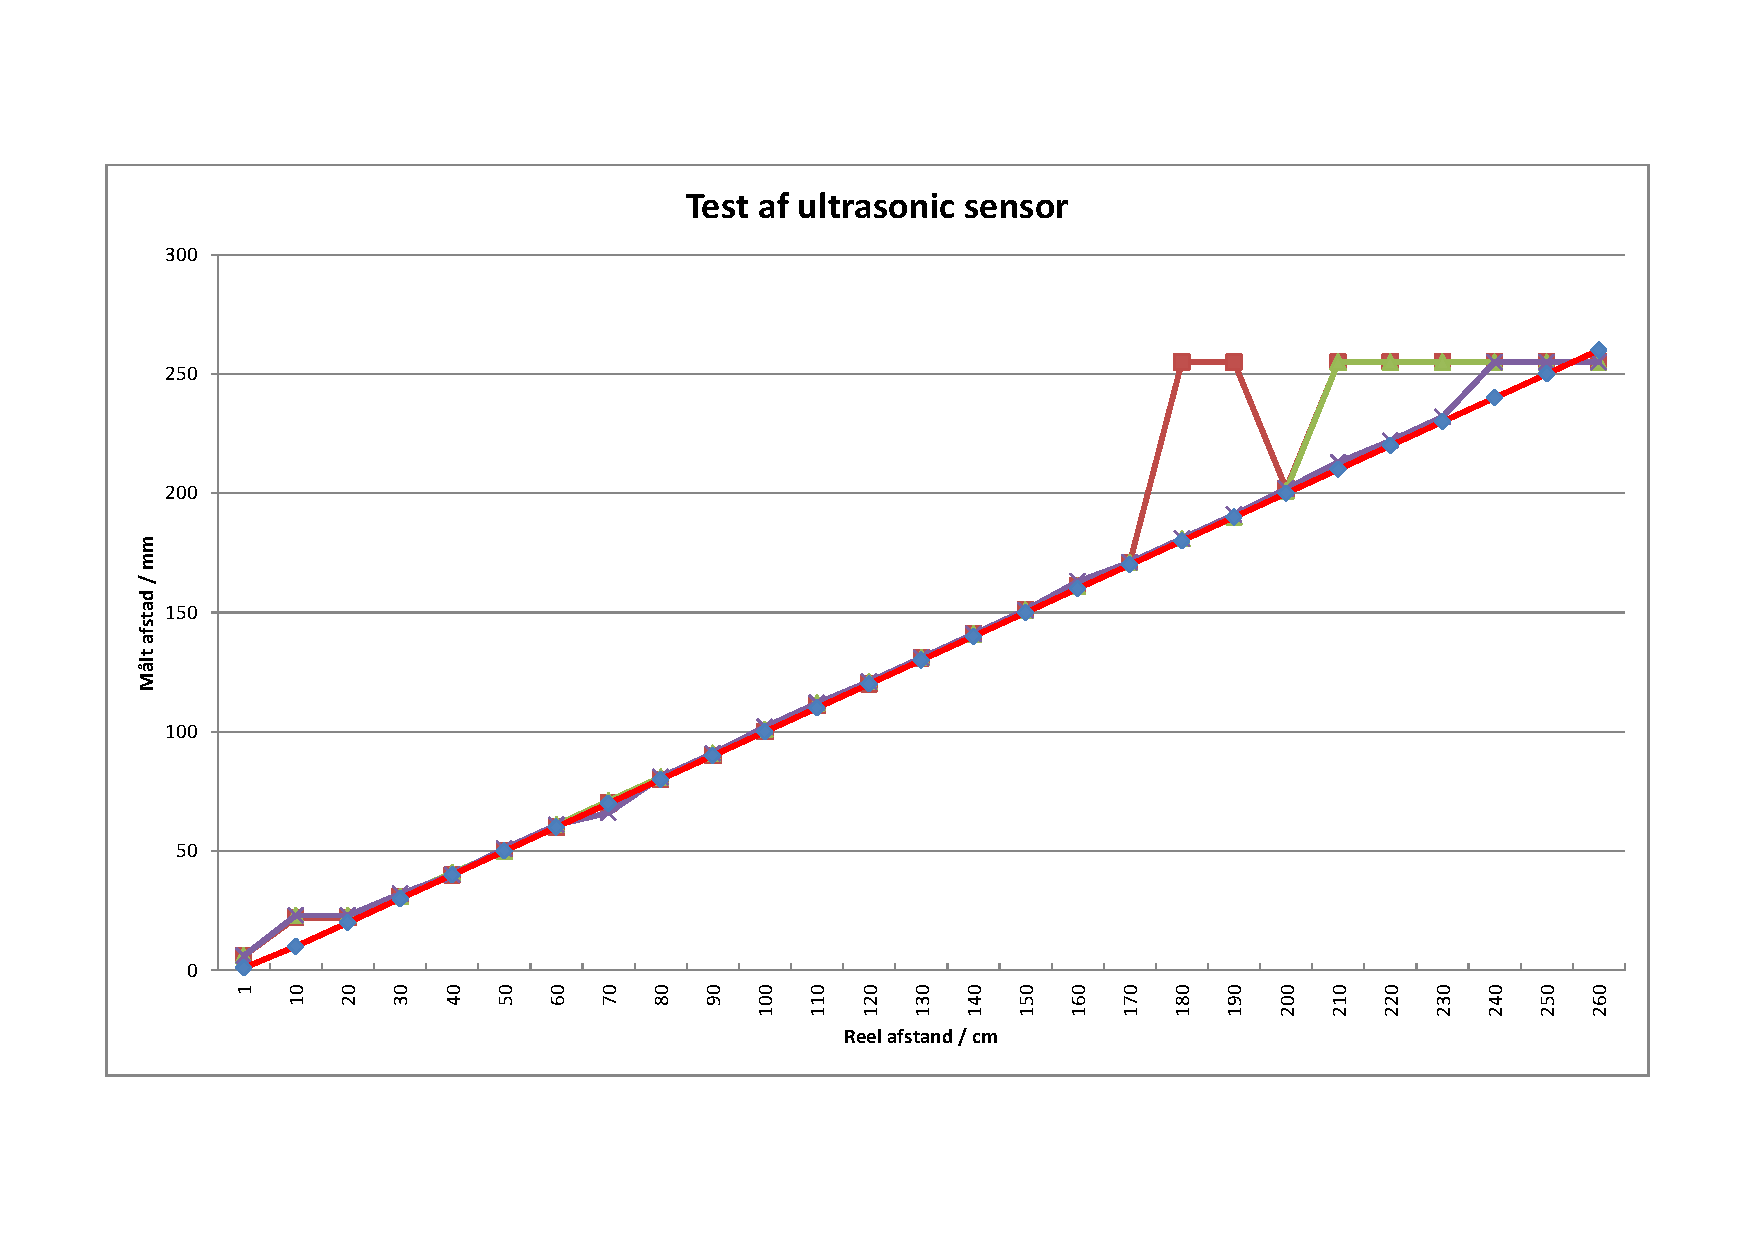
\includegraphics[width=\textwidth]{ultrasonicchart}
\caption{Graf over forsøgsresultaterne fra testen af den ultrasoniske sensor}
\label{sensor:ultrasonic_resultat_diagram}
\end{figure}



\subsection{Infrarød Sensor}
Den infrarøde afstandssensor fra mindsensors.com, som kan ses på \cref{sensor:infraroed_sensor}, er en afstandssensor med høj præcision og måler afstande mellem 10 og 80 cm.
Sensoren virker som ultrasonisk sensoren, men sender et infrarødt signal i stedet for en ultrasonisk impuls.\cite{infrared}

\subsubsection{Formål}
Formålet med at teste denne sensor er, at robotten skal have en måde at afgøre på, hvor langt der er til objekter omkring den.
Derfor vil denne test undersøge følgende:
\begin{itemize}
\item Hvor nøjagtigt kan denne sensor bestemme afstanden til et objekt?
\item Hvilket interval kan der måles i, hvad er den minimale og maksiamle måleafstand?
\end{itemize}

\subsubsection{Test}
For at afprøve sensorens præcision og rækkevidde er der foretaget en test af sensoren.

Opstillingen brugt til udførelse af testen bestod af tre A4 ark spændt ud på gulvet ind til en væg. 
Papiret havde markeringer for hver 2 cm fra væggen.

Udførelsen af testen gik ud på at placere en NXT med påsat infrarød sensor ved hver indikator, for derefter at aflæse sensorens måling.
På denne måde blev afmålingen fra sensoren ved en given afstand holdt op imod den egentlige afstand til væggen, som afmålt på papiret.

\subsubsection{Resultater}

Resultaterne fra testen er præsenteret i \cref{appendix:infrared}. 
Disse resultater er sat op i et diagram i \cref{sensor:infrared_chart}.
Den røde graf er den reelle afstand, som aflæst på papiret/med lineal, mens de blå firkanter er målepunkter.
Den sorte graf er en lineær regression over måleresultaterne.

Ud fra grafen kan det ses at der er stor usikkerhed i starten og slutningen, hvilket næsten stemmer overens med den lovede rækkevidde på 10 til 80 cm.
De bedste resultater findes dog imellem 8cm og 56 cm. 
Mellem 8cm og 56cm er der maximalt 27 mm afvigelse fra det forventede, (forventet 500, målt 527).

\begin{figure}[h]
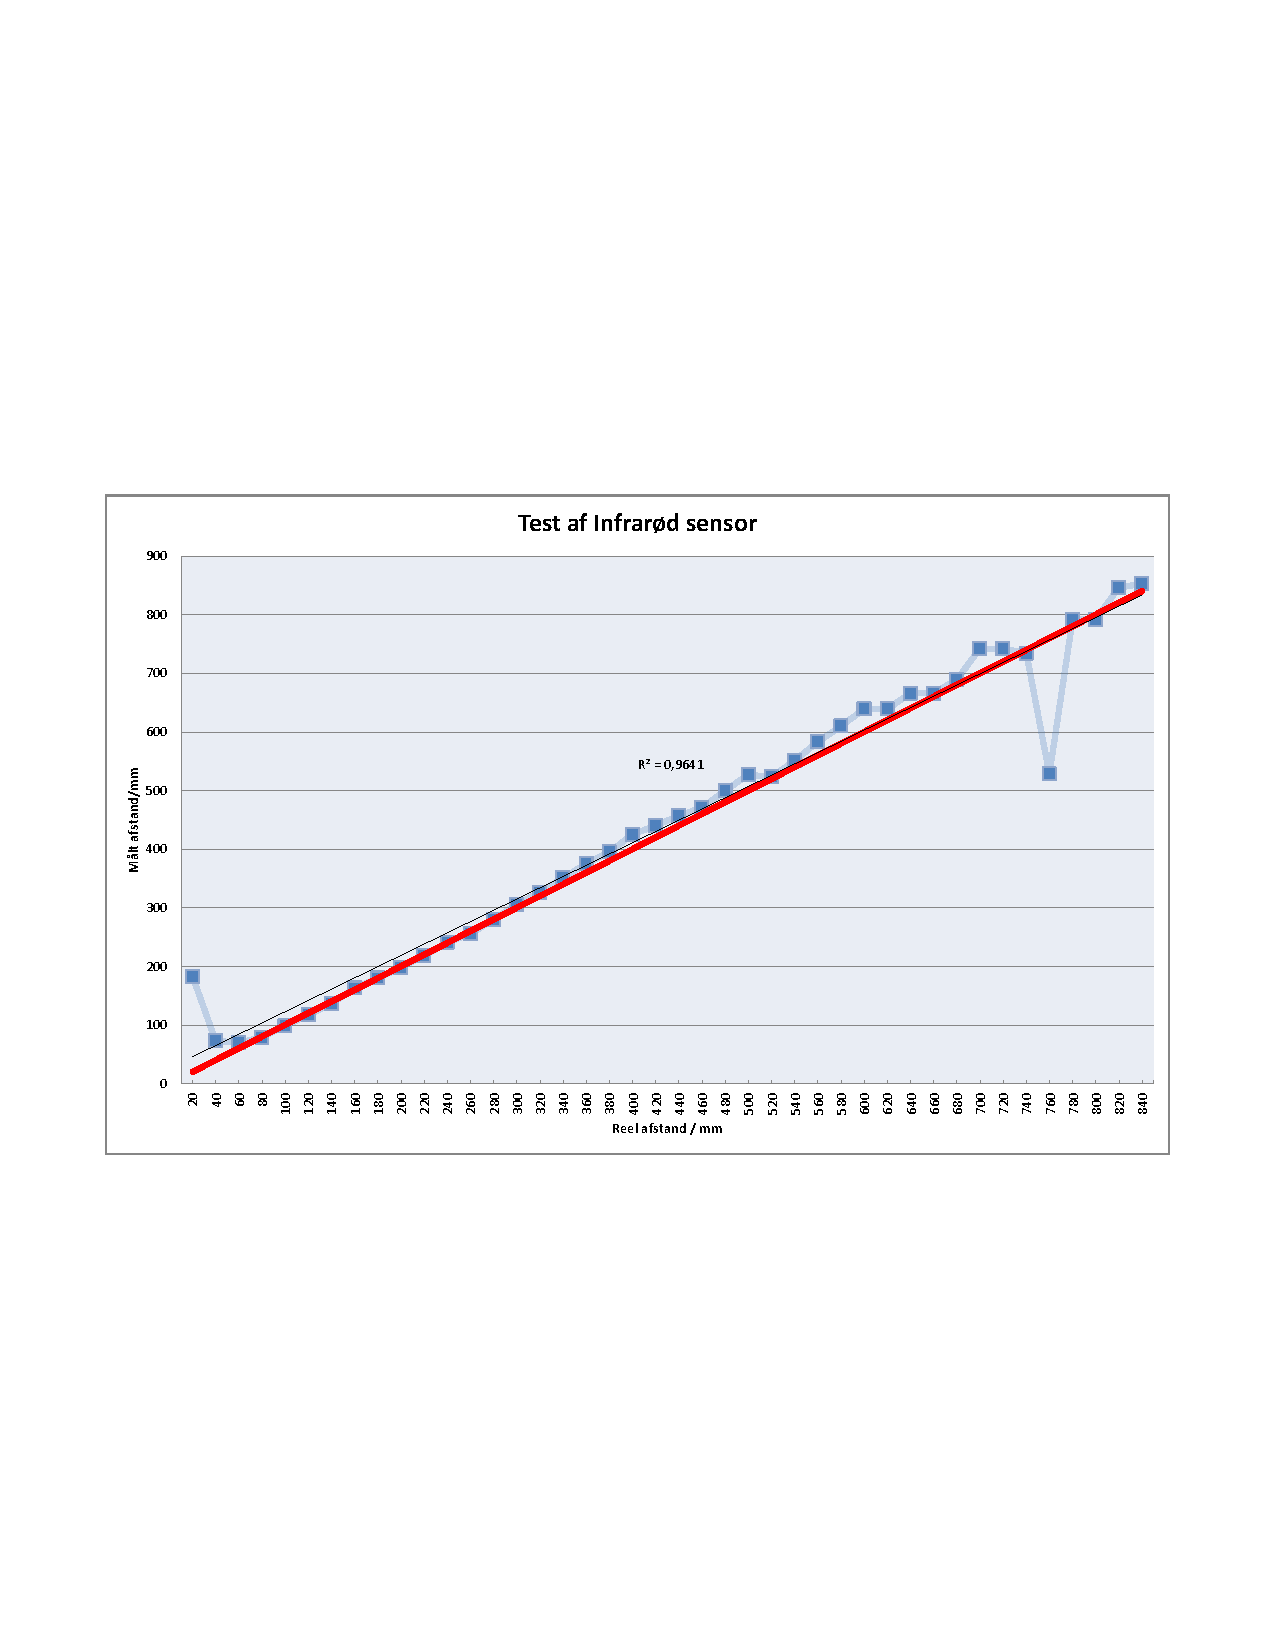
\includegraphics[width=\textwidth]{Infraredchart}
\caption{Graf over forsøgsresultaterne fra testen af den infrarøde sensor}
\label{sensor:infrared_chart}
\end{figure}

\subsection{Sammenligning af afstandssensorer}

Der er nu foretaget test af to forskellige afstandssensorer, den ultrasoniske sensor og den infrarøde sensor. 
Den ultrasoniske sensor var præcis med en afvigelse på $\pm$3 cm mellem 20 cm og 170 cm.
Den infrarøde sensor var præcis med afvigelse på $\pm$3 cm, mellem 10 cm og 56 cm.
Den infrarøde sensor angiver sine målinger med højere præcision, men da fejlmarginen er 3 cm anses den ikke som værende mere præcis end den ultrasoniske sensor.
I forhold til afstand, måler den ultrasoniske længere væk end den infrarøde, mens den infrarøde sensor måler tættere på end den ultrasoniske.
Valget mellem de to sensorer står derfor på hvilket krav robotten har til afstand.

\subsection{Motor}\label{sensorer:motorer}
Motoren beskrevet i dette afsnit er \lego's egen.
Den består af en rotationssensor som måler omdrejningerne ved grader med en nøjagtighed på 1 grad, hvilket er med til at gøre motoren ret præcis. 
Desuden gør denne sensor det også muligt at styre hvor meget kraft motoren skal køre med.
Køres der med flere motorer har NXT'en indbygget software der gør det muligt at synkronisere disse, hvilket er smart hvis den ene motor skulle være stærkere eller svagere end den anden.\cite{tikNXT}
Motoren kan ses på \cref{sensor:motor_sensor}.
\mikkel{Ovenstående skal skrives om - jeg nåede det bare ikke inden vi sendte til vejleder}

\subsubsection{Formål}
Formålet med denne test er at undersøge hvorvidt denne motor kan bruges til projektets robot.
Det er interessant at afklare hvorvidt de kan styres med \'en grads præcision.

\subsubsection{Test}
For at bestemme motorens nøjagtighed i praksis, blev en test opstillet hvor to moterer roteres med et bestemt antal grader.
Motorernes egentlige rotation aflæses med vinkelmåler og holdes op mod den ønskede rotation, samt den rotation motorerne angiver at de har roteret.
Sidstenævnte fås ved at aflæse motorernes \lstinline[style=csharp]!TachoCount! egenskab.

\paragraph{Resultaterne} fra forsøget kan ses i \cref{sensor:motor_test_data} på side \pageref{sensor:motor_test_data}.
\mikkel{Der er nogle fejl i dette afsnit som skal rettes efter vi har sendt til vejleder}
Af resultaterne kan vi bestemme den største afvigelse til +7 og -4 grader målt.
Tacho-værdien har en afvigelse på maksimalt +1 og -4 grader.
Dette stemmer ikke overens med de antagede $\pm$1 grad afvigelse.

+7 og +6 grader målt optræder kun en gang.
Ellers er den maksimale målte afvigelse $\pm$4 grader, men selvom vi antager at det er pga. unøjagtige målinger ved forsøgsudførelsen, er det stadig ikke $\pm$1 grad.
\stefan{Man kan ikke direkte aflæse afvigelserne fra tabellen}
\thilemann{Synes heller ikke meningen står helt klar}
Kigger vi på \cref{sensor:motor_sensor_diagram} kan vi se at målingerne ligger længst udenfor det optimale (sorte stiplede linje), hvilket er en god indikator på at det er bedre at benytte tacho-værdien.

\begin{figure}
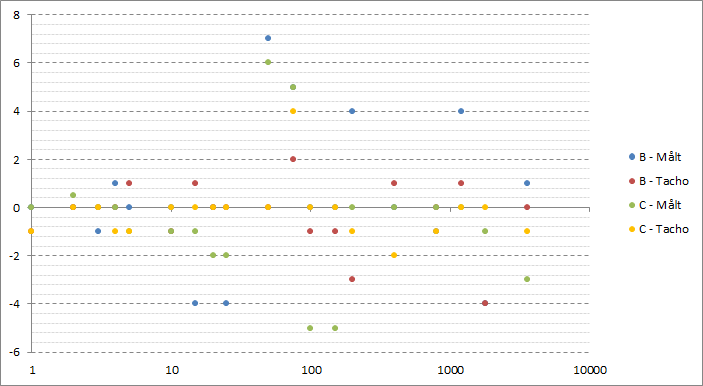
\includegraphics{motor_diagram}
\caption{Afvigelser i test-resultaterne}
\label{sensor:motor_sensor_diagram}
\end{figure}

Desuden kan vi se på samme figur at motor b er meget mere unøjagtig end motor c.
Ideelt ville de to motorer give det samme resultat.

Dvs. den målte værdi har en afvigelse på $\pm$4 grader, mens tacho-værdien har en afvigelse på +1 og -4 grader, og at synkronisering af de to motrer ikke giver den ønskede effekt.
